
% This LaTeX was auto-generated from MATLAB code.
% To make changes, update the MATLAB code and republish this document.

\documentclass{article}
\usepackage{graphicx}
\usepackage{color}

\sloppy
\definecolor{lightgray}{gray}{0.5}
\setlength{\parindent}{0pt}

\begin{document}

    
    

\section*{20. Caratheodory--Fejer approximation}

\begin{verbatim}
ATAPformats
\end{verbatim}
\begin{par}
 We have seen that Chebyshev interpolants are near-best
approximations in the sense that they come within a factor of at most
$O(\log n)$ of best approximations, usually even closer. For most
applications, this is all one could ask for.  But there is another kind
of near-best approximations that are so close to best that for smooth
functions, they are often indistinguishable from best approximations to
machine precision on a computer.  These are {\em CF
(Carath\'eodory--Fej\'er) approximations}, introduced by Gutknecht and
Trefethen [1982]. Earlier related ideas were proposed in [Darlington
1970, Elliott 1973, Lam 1972, Talbot 1976], and the theoretical basis
goes back to the early 20th century [Carath\'eodory \& Fej\'er 1911,
Schur 1918].\footnote{Logically, this chapter could have appeared
earlier, perhaps just after Chapter 10.  We have deferred it to this
point of the book, however, since the material is relatively difficult
and none of the other chapters depend on it.} 
\end{par} \vspace{1em}
\begin{par}
Before explaining the mathematics of CF approximants, let us illustrate the remarkable degree of near-optimality they sometimes achieve.  Here is the optimal $\infty$-norm error in approximation of $f(x) = e^x$ on $[-1,1]$ by a polynomial of degree 2:
\end{par} \vspace{1em}
\begin{par}
 \vskip -2em 
\end{par} \vspace{1em}
\begin{verbatim}
x = chebfun('x'); format long
f = exp(x); n = 2;
pbest = remez(f,n);
errbest = norm(f-pbest,inf)
\end{verbatim}

        \color{lightgray} \begin{verbatim}errbest =
   0.045017388402819
\end{verbatim} \color{black}
    \begin{par}
Here is the corresponding error for CF approximation computed by the Chebfun \texttt{cf} command:
\end{par} \vspace{1em}
\begin{par}
 \vskip -2em 
\end{par} \vspace{1em}
\begin{verbatim}
pcf = cf(f,n);
errcf = norm(f-pcf,inf)
\end{verbatim}

        \color{lightgray} \begin{verbatim}errcf =
   0.045017388414604
\end{verbatim} \color{black}
    \begin{par}
These two numbers agree to an extraordinary 9 significant digits. Comparing the best and CF polynomials directly to one another, we confirm that they are almost the same:
\end{par} \vspace{1em}
\begin{par}
 \vskip -2em 
\end{par} \vspace{1em}
\begin{verbatim}
norm(pbest-pcf,inf)
\end{verbatim}

        \color{lightgray} \begin{verbatim}ans =
     1.178523945100096e-11
\end{verbatim} \color{black}
    \begin{par}
That was for degree $n=2$, and the near-optimality of the CF approximants grows stronger as $n$ increases. Let us explore the dependence on $n$. On a semilog plot, the upper curve in the next figure shows the accuracy of the best polynomial as an approximation to $f(x)$, while the lower curve shows the accuracy of the CF polynomial as an approximation to the best polynomial. The two errors are of entirely different orders, and for $n> 3$, the CF and best polynomials are indistinguishable in floating point arithmetic.
\end{par} \vspace{1em}
\begin{par}
 \vskip -2em 
\end{par} \vspace{1em}
\begin{verbatim}
nn = 0:10; err1 = []; err2 = [];
for n = nn
    pbest = remez(f,n); err1 = [err1 norm(f-pbest,inf)];
    pcf = cf(f,n); err2 = [err2 norm(pbest-pcf,inf)];
end
hold off, semilogy(nn,err1,'.-'), grid on
hold on, semilogy(nn,err2,'.-r')
FS = 'fontsize';
text(7.5,2e-6,'f-p_{best}','color','b',FS,10)
text(1.2,1e-14,'p_{best}-p_{CF}','color','r',FS,10)
ylim([1e-18,1e2]), xlabel('n',FS,9)
title(['For smooth functions, ' ...
     'CF approx is almost the same as best approx'],FS,9)
\end{verbatim}

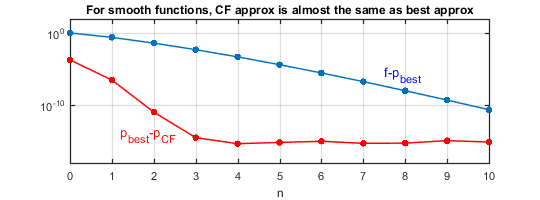
\includegraphics [width=4in]{chap20_01.png}
\begin{par}
 \vskip 1pt 
\end{par} \vspace{1em}
\begin{par}
Here is the same experiment repeated for $f(x) = \tanh(4(x-0.3))$.
\end{par} \vspace{1em}
\begin{par}
 \vskip -2em 
\end{par} \vspace{1em}
\begin{verbatim}
f = tanh(4*(x-.3));
nn = 0:30; err1 = []; err2 = [];
for n = nn
    pbest = remez(f,n); err1 = [err1 norm(f-pbest,inf)];
    pcf = cf(f,n); err2 = [err2 norm(pbest-pcf,inf)];
end
hold off, semilogy(nn,err1,'.-'), grid on
hold on, semilogy(nn,err2,'.-r')
text(16,2e-2,'f-p_{best}','color','b',FS,10)
text(5.3,1e-13,'p_{best}-p_{CF}','color','r',FS,10)
ylim([1e-18,1e2]), xlabel('n',FS,9)
title('Same curves for another function f',FS,9)
\end{verbatim}

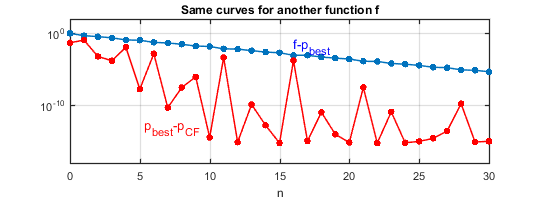
\includegraphics [width=4in]{chap20_02.png}
\begin{par}
 \vskip 1pt 
\end{par} \vspace{1em}
\begin{par}
Again we see that \texttt{pbest} $\!\!-\!\!$ \texttt{pcf} is much smaller than \texttt{f} $\!\!-\!\!$ \texttt{pbest}, implying that the CF approximant is for practical purposes essentially optimal.  (Concerning the erratic oscillations, see Exercise 20.4.) Yet it is far easier to compute:
\end{par} \vspace{1em}
\begin{par}
 \vskip -2em 
\end{par} \vspace{1em}
\begin{verbatim}
tic, remez(f,20); tbest = toc
tic, cf(f,20); tcf = toc
\end{verbatim}

        \color{lightgray} \begin{verbatim}tbest =
   0.140552533721746
tcf =
   0.010225742811077
\end{verbatim} \color{black}
    \begin{par}
Turning to a non-smooth function, here again is the jagged example from Chapter 10 with its best approximation of degree 20:
\end{par} \vspace{1em}
\begin{par}
 \vskip -2em 
\end{par} \vspace{1em}
\begin{verbatim}
f = cumsum(sign(sin(20*exp(x))));
hold off, plot(f,'k'), grid on
tic, [pbest,err] = remez(f,20); tbest = toc;
hold on, plot(pbest)
title('Jagged function and best approximation',FS,9)
\end{verbatim}

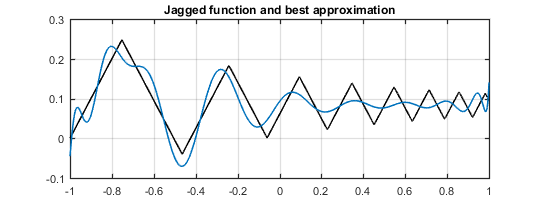
\includegraphics [width=4in]{chap20_03.png}
\begin{par}
 \vskip 1pt 
\end{par} \vspace{1em}
\begin{par}
We saw the error curve before:
\end{par} \vspace{1em}
\begin{par}
 \vskip -2em 
\end{par} \vspace{1em}
\begin{verbatim}
hold off, plot(f-pbest), grid on, hold on, axis([-1 1 -.08 .08])
plot([-1 1],err*[1 1],'--k'), plot([-1,1],-err*[1 1],'--k')
title('Best approximation error curve',FS,9)
\end{verbatim}

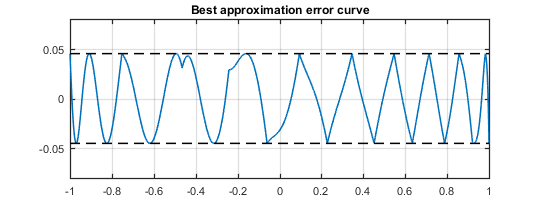
\includegraphics [width=4in]{chap20_04.png}
\begin{par}
 \vskip 1pt 
\end{par} \vspace{1em}
\begin{par}
In CF approximation, we must start from a polynomial, not a jagged function.  As a rule of thumb, truncating the Chebyshev series at 5 times the degree of the desired approximation is usually pretty safe.  Here is what we get:
\end{par} \vspace{1em}
\begin{par}
 \vskip -2em 
\end{par} \vspace{1em}
\begin{verbatim}
f100 = chebfun(f,100);
tic, pcf = cf(f100,20); tcf = toc;
hold off, plot(f-pcf), grid on, hold on, axis([-1 1 -.08 .08])
plot([-1 1],err*[1 1],'--k'), plot([-1,1],-err*[1 1],'--k')
title('CF approximation error curve',FS,9)
\end{verbatim}

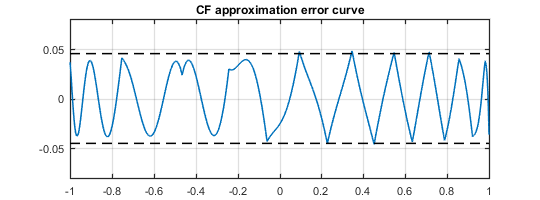
\includegraphics [width=4in]{chap20_05.png}
\begin{par}
 \vskip 1pt 
\end{par} \vspace{1em}
\begin{par}
Evidently the error falls short of optimality by just a few percent. Yet again the computation is much faster:
\end{par} \vspace{1em}
\begin{par}
 \vskip -2em 
\end{par} \vspace{1em}
\begin{verbatim}
tbest
\end{verbatim}

        \color{lightgray} \begin{verbatim}tbest =
   1.373288030369765
\end{verbatim} \color{black}
    \begin{verbatim}
tcf
\end{verbatim}

        \color{lightgray} \begin{verbatim}tcf =
   0.013967521273695
\end{verbatim} \color{black}
    \begin{par}
Here for comparison is the error in Chebyshev interpolation.
\end{par} \vspace{1em}
\begin{par}
 \vskip -2em 
\end{par} \vspace{1em}
\begin{verbatim}
pinterp = chebfun(f,21);
hold off, plot(f-pinterp), grid on, hold on, axis([-1 1 -.08 .08])
plot([-1 1],err*[1 1],'--k'), plot([-1,1],-err*[1 1],'--k')
title('Chebyshev interpolation error curve',FS,9)
\end{verbatim}

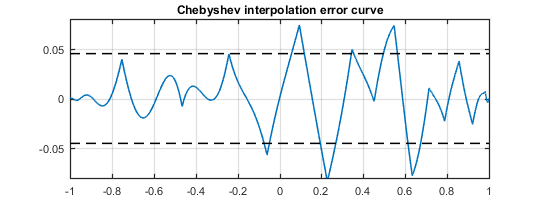
\includegraphics [width=4in]{chap20_06.png}
\begin{par}
 \vskip 1pt 
\end{par} \vspace{1em}
\begin{par}
The time has come to describe what CF approximation is all about. We shall see that the hallmark of this method is the use of eigenvalues and eigenvectors (or singular values and singular vectors) of a Hankel matrix of Chebyshev coefficients.
\end{par} \vspace{1em}
\begin{par}
We start with a real function $f$ on $[-1,1]$, which we want to approximate by a polynomial of degree $n\ge 0$. Following Theorem 3.1, we assume that $f$ is Lipschitz continuous, so it has an absolutely convergent Chebyshev series $$ f(x) = \sum_{k=0}^\infty  a_k T_k(x). $$ Since our aim is polynomial approximation, there is no loss of generality if we suppose that $a_0 = a_1 = \cdots = a_n = 0$, so that the Chebyshev series of $f$ begins at the term $T_{n+1}$.  For technical simplicity, let us further suppose that the series is a finite one, ending at the term $T_N$ for some $N \ge n+1$.  Then $f$ has the Chebyshev series $$ f(x) = \sum_{k=n+1}^N  a_k T_k(x). $$ We now transplant $f$ to a function $F$ on the unit circle in the complex $z$-plane by defining $F(z) = F(z^{-1}) = f(x)$ for $|z|=1$, where $x = \hbox{Re}\,z = (z+z^{-1})/2$. As in the proof of Theorem 3.1, this gives us a formula for $F$ as a Laurent polynomial, $$ F(z) = {1\over 2} \sum_{k=n+1}^N a_k (z^k + z^{-k}). $$ We can divide $F$ into two parts, $F(z) = G(z) + G(z^{-1})$, with $$ G(z) = {1\over 2} \sum_{k=n+1}^N a_k z^k. $$ The function $G$ is called the \textit{analytic part} of $F$, since it can be analytically continued to an analytic function in $|z|\le 1$.  Similarly $G(z^{-1})$ is the \textit{coanalytic part} of $F$, analytic for $1 \le |z|\le \infty$.
\end{par} \vspace{1em}
\begin{par}

Now we ask the following question: what is the best
approximation $\tilde P$ to $G$ on the unit circle of the form
$$ \tilde P(z) = {1\over 2} \sum_{k=-\infty}^n b_k z^k, \eqno (20.1) $$
where the series converges for all $z$ with $1\le |z| < \infty$? In other
words, $\tilde P$ must be analytic in the exterior of the unit disk apart
from a pole of order at most $n$ at $z=\infty$. This is the problem that
Carath\'eodory and Fej\'er solved, and the solution is
elegant.  First of all, $\tilde P$ exists, and it is unique.  Secondly,
$G-\tilde P$ maps the unit circle onto a perfect circle that winds
counterclockwise around the origin a number of times: the winding number
is at least $n+1$.  Third, as shown by Schur a few years after
Carath\'eodory and Fej\'er [Schur 1918], $\tilde P$ can
be constructed explicitly by solving a certain matrix singular value
problem.  Let $H$ denote the $(N-n)\times (N-n)$ real symmetric matrix of
Chebyshev coefficients arranged like this,
$$ H = \pmatrix{ a_{n+1} & a_{n+2} & a_{n+3} & \dots & a_N \cr\noalign{\vskip 3pt}
a_{n+2} & a_{n+3} & \cr\noalign{\vskip 3pt} a_{n+3} \cr\noalign{\vskip 3pt} \vdots \cr\noalign{\vskip 3pt}  a_N }, \eqno (20.2) $$
where the entries in the lower-right triangle are zero. A matrix with
this structure, constant along diagonals so that $a_{ij}$ depends only on
$i+j$, is called a {\em Hankel matrix}. Let $\lambda$ be the largest
eigenvalue of $H$ in absolute value, let $u = (u_0, u_1, \dots ,
u_{N-n-1})^T$ be a corresponding real eigenvector, and define
$$ u(z) = u_0^{} + u_1^{} z + \cdots + u_{N-n-1}^{}z^{N-n-1}. $$
Here is the theorem due to
Carath\'eodory and Fej\'er and Schur.

\end{par} \vspace{1em}
\begin{par}
\textbf{Theorem 20.1. $\hbox{Carath\'eodory--Fej\'er--Schur}$ theorem}. \textit{The approximation problem described above has a unique solution $\tilde P$, and it is given by the error formula} $$ (G-\tilde P)(z) = \lambda \kern 1pt z^{n+1} \kern 1pt {u(z)\over \,\overline{u(z)}\,}. \eqno (20.3) $$ \textit{The function $G-\tilde P$ maps the unit circle to a circle of radius $|\lambda|$ and winding number $\ge n+1$, and if $|\lambda|>|\mu|$ for all other eigenvalues $\mu$, the winding number is exactly $n+1$.}
\end{par} \vspace{1em}
\begin{par}
\textit{Proof.}  The result is due to $\hbox{Carath\'eodory and Fej\'er}$ [1911] and Schur [1918].  See Theorem 1.1 of [Gutknecht \& Trefethen 1982] and Theorem 4 of [Hayashi, Trefethen \& Gutknecht 1990]. $~\hbox{\vrule width 2.5pt depth 2.5 pt height 3.5 pt}$
\end{par} \vspace{1em}
\begin{par}

Theorem 20.1 is a mathematical assertion about the approximation of a
function $G$ on the unit circle by an infinite series. We use this result
to construct the polynomial CF approximant as follows. Since $G-\tilde P$
maps the unit circle to a circle of winding number $\ge n+1$, its real
part (times 2)
$$ (G-\tilde P)(z) + (G-\tilde P)(z^{-1}) $$
maps $[-1,1]$ to an equioscillating curve with at least
$n+2$ extreme points.  Thus the function
$$ \tilde p(x) = \tilde P(z) + \tilde P(z^{-1}) $$
yields the equioscillatory behavior that characterizes a best
approximation polynomial of degree $n$ to $f(x)$ on $[-1,1]$ (Theorem
10.1). Unfortunately, $\tilde p(x)$ is not a polynomial of degree $n$.
However, it will generally be very close to one.  The function $\tilde P$
will normally have Laurent series coefficients $b_k$ that decay as
$k\to-\infty$.  We truncate these at degree $-n$ to define
$$ {\cal P}_{\hbox{\tiny CF}}^{}(z) = {1\over 2} \sum_{k=-n}^n b_k z^k, $$
with real part (times 2)
$$ p_{\hbox{\tiny CF}}^{}(x) =
{\cal P}_{\hbox{\tiny CF}}^{}(z) + {\cal P}_{\hbox{\tiny CF}}^{}(z^{-1})
= {1\over 2} \sum_{k=-n}^n (b_k + b_{-k}) z^k. $$ If the truncated terms
are small, $f-p_{\hbox{\tiny CF}}^{}$ maps $[-1,1]$ to a curve that comes
very close to equioscillation with $\ge n+2$ extrema, and thus
$p_{\hbox{\tiny CF}}^{}$ is close to optimal.

\end{par} \vspace{1em}
\begin{par}
For more details on real polynomial CF approximation, with numerical examples, see [Gutknecht \& Trefethen 1982], [Trefethen 1983], and [Hayashi, Trefethen \& Gutknecht 1990].
\end{par} \vspace{1em}
\begin{par}
Our experiments in the opening pages of this chapter showed that CF approximants can be exceedingly close to best.  The truncation described above gives an idea of how this happens.  In the simplest case, suppose $f$ is an analytic function on $[-1,1]$.  Then by Theorem 8.1, its Chebyshev coefficients decrease geometrically, and let us suppose that this happens smoothly at a rate $a_k = O(\rho^k)$.  Then, roughly speaking, the dominant degree $n+1$ term of $f$ is of order $\rho^{-n-1}$, and the terms $b_n, b_{n-1}, \dots, b_{-n}$ are of orders $\rho^{-n-2},\rho^{-n-3},\dots, \rho^{-3n-2}$.  This suggests that the truncation in going from $\tilde p$ to $p_{\hbox{\tiny CF}}^{}$ will introduce an error of order $\rho^{-3n-3}$.  This is usually a very small number, and in particular, much smaller than the error $\|f-p^*\|$ of order $\rho^{-n-1}$.
\end{par} \vspace{1em}
\begin{par}
In fact, the actual order of accuracy for polynomial CF approximation is one order higher, $\rho^{-3n-4}$ rather than $\rho^{-3n-3}$.  (The reason is that the first truncated term is a multiple of $T_{3n+3}$, the same Chebyshev polynomial that dominates the error $f-p^*$ itself, and so it is not until the second truncated term, $T_{3n+4}$, that the equioscillation is broken.)  On the other hand, to go from this rough argument to a precise theorem is not so easy, because in fact, Chebyshev series need not decay smoothly (Exericse 20.3). Here we quote without proof a theorem from [Gutknecht \& Trefethen 1982].
\end{par} \vspace{1em}
\begin{par}

{\em{\bf Theorem 20.2. Accuracy of polynomial CF approximation.} For any fixed
$m\ge 0$, let $f$ have a Lipschitz continuous $(3m+3)$rd derivative on
$[-1,1]$ with a nonzero $(m+1)$st derivative at $x=0$, and for each $s\in
(0,1]$, let $p^*$ and $p_{\hbox{\tiny CF}}^{}$ be the best and the CF
approximations of degree $m$ to $f(sx)$ on $[-1,1]$, respectively. Then
as $s\to 0$,
$$ \|f-p^*\| = O(s^{m+1}) \eqno (20.4) $$
and
$$ \|f-p^*\| \ne O(s^{m+2}) \eqno (20.5) $$
and
$$ \|\kern .7pt p_{\hbox{\tiny CF}}^{}-p^*\| = O(s^{3m+4}). \eqno (20.6) $$
}

\end{par} \vspace{1em}
\begin{par}
\textit{Proof.}  See Theorem 3.4 of [Gutknecht \& Trefethen 1982]. $~\hbox{\vrule width 2.5pt depth 2.5 pt height 3.5 pt}$
\end{par} \vspace{1em}
\begin{par}
We can verify this result numerically.  The two plots below display norms for $m=1$ and $m=2$ for the function $f(x) = e^{5x}$.
\end{par} \vspace{1em}
\begin{par}
 \vskip -2em 
\end{par} \vspace{1em}
\begin{verbatim}
ff = @(x) exp(5*x);
for m = 1:2
  ss = .8.^(0:20); errfp = []; errpp = [];
  for s = ss
    f = chebfun(@(x) ff(s*x));
    pbest = remez(f,m); pcf = cf(f,m);
    errfp = [errfp norm(f-pbest,inf)];
    errpp = [errpp norm(pcf-pbest,inf)];
  end
  hold off, loglog(ss,errfp,'.-')
  hold on, loglog(ss,errpp,'.-r'), loglog(ss,ss.^(m+1),'--');
  s = 0.025; text(s,.1*s^(m+1)/4,'s^{m+1}','color','b',FS,10)
  loglog(ss,ss.^(3*m+4),'--r')
  text(s,.02*s^(3*m+4)*1e4,'s^{3m+4}','color','r',FS,10)
  text(.015,.01+(2-m)*.5,'f-p_{best}','color','b',FS,10)
  text(.25,1e-12+(2-m)*1e-8,'p_{best}-p_{CF}','color','r',FS,10)
  axis([1e-2 1 1e-18 1e3]), xlabel('s',FS,9), ylabel error
  title(['Convergence for m = ' int2str(m)],FS,9), snapnow
end
\end{verbatim}

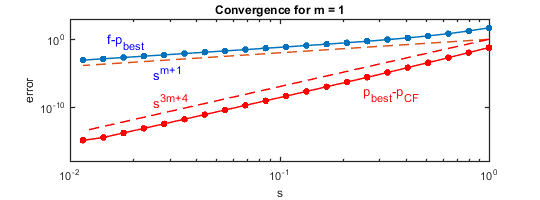
\includegraphics [width=4in]{chap20_07.png}

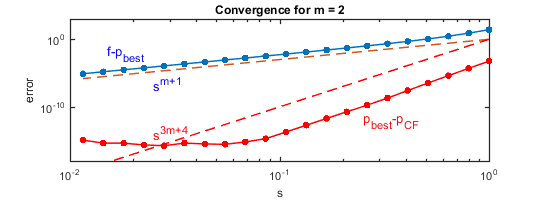
\includegraphics [width=4in]{chap20_08.png}
\begin{par}
 \vspace{1pt} 
\end{par} \vspace{1em}
\begin{par}
In this chapter we have considered CF approximation in its simplest context of approximation of one polynomial $f$ of degree $N$ by another polynomial $p_{\hbox{\tiny CF}}^{}$ of degree $n$.  In fact, the method is much more general.  So long as $f$ has an absolutely convergent Chebyshev series, which is implied for example if it is Lipschitz continuous, then Theorem 20.1 still applies [Hayashi, Trefethen \& Gutknecht 1990]. Now $H$ is an infinite matrix which can be shown to represent a compact operator on $\ell^2$ or $\ell^1$, its dominant eigenvector is an infinite vector, and $u(z)$ is defined by an infinite series.  The error curve is still a continuous function of winding number at least $n+1$.
\end{par} \vspace{1em}
\begin{par}
Another generalization is to approximation by rational functions rather than polynomials.  Everything goes through in close analogy to what has been written here, and now the other eigenvalues of the Hankel matrix come into play.  The theoretical underpinnings of rational CF approximation can be found in papers of Takagi [1924], Adamyan, Arov and Krein [1971], and Trefethen and Gutknecht [1983b], as well as the article by Hayashi, Trefethen and Gutknecht cited above. Quite apart from theory, one can compute these approximations readily by the Chebfun \texttt{cf} command using capabilities introduced by Joris Van Deun.  For details and examples see [Van Deun \& Trefethen 2011].
\end{par} \vspace{1em}
\begin{par}

Further generalizations of CF approximation concern approximation of vector or matrix
functions rather than just scalars, and here, such techniques are
associated with the name {\em $H^\infty$ approximation}.  An important early
paper was Glover [1984], and there have been many extensions and generalizations
since then [Antoulas 2005, Zhou, Doyle \& Glover 1996].

\end{par} \vspace{1em}
\begin{par}

We have emphasized the practical power of CF approximants as
providing near-best approximations at low computational cost.
The conceptual and theoretical significance of the technique, however, goes
beyond this.  Indeed, the eigenvalue/singular value analysis of
Carath\'eodory--Fej\'er approximation seems to be the principal known
algebraic window into the detailed analysis of best approximations, and
in most cases where best approximations of a function happen to be
known exactly, these best approximations are CF approximations in which
an approximant like $\tilde P$ or $\tilde p$ already has the required finite
form, so that nothing must be truncated to get to $P$ or $p$ [Gutknecht 1983].

\end{par} \vspace{1em}
\begin{par}

\begin{displaymath}
\framebox[4.7in][c]{\parbox{4.5in}{\vspace{2pt}\sl
{\sc Summary of Chapter 20.}
Carath\'eodory--Fej\'er approximation constructs near-best
approximations of a function $f\in C([-1,1])$ from the singular values
and vectors of a Hankel matrix of Chebyshev coefficients. If $f$ is
smooth, CF approximants are often indistinguishable in machine precision
from true best approximants.\vspace{2pt}}}
\end{displaymath}

\end{par} \vspace{1em}
\begin{par}
 \small\smallskip\parskip=2pt
{\bf Exercise 20.1.  Approximating \boldmath$\cos(nx)$.}
(a) For $n = 2,4,8,16,\dots,$ compute the degree $n$ CF approximant
to $f(x) = \cos(nx)$ and plot the error curve.  How high can you go in
this sequence?
(b) What happens if $\cos(nx)$ is changed to $\cos(0.9\kern .7pt nx)$?
\par
{\bf Exercise 20.2.  Approximating the jagged function.} Four of the
figures of this chapter concerned approximations of degree 20 to a jagged
function.  (a) How do the $L^2$ norms of the best and CF approximations
compare?  (b) The CF approximation was based on truncation of the
Chebyshev series at term $N=100$.  How does the $\infty$-norm of the
error vary with $N$?
(c) Draw a conclusion from this exploration: is the imperfect
equioscillation of the error curve in the figure given in the text for
this function mostly to the fact that CF approximation is not best
approximation, or to the fact that $N <\infty$?
\par
{\bf Exercise 20.3.  Complex approximation on the unit disk.} (a) Suppose
$f$ is an analytic function on the closed unit disk and $p$ is a
polynomial of degree $n$.  Prove that $p$ is a best approximation to $f$
in the $\infty$-norm on the disk $|z|\le 1$ if and only if it is a best
approximation on the circle $|z|=1$.
(b) Look up $\hbox{Rouch\'e's}$ theorem and write down a careful
statement, citing your source. (c) Suppose $f$ is an analytic function in
the closed unit disk and $p$ is a polynomial of degree $n$ such that
$f-p$ maps the unit circle to a circle of winding number at least $n+1$.
Prove that $p$ is a best approximation to $f$ on the unit disk. (In fact
it is unique, though this is not obvious.)
\par
{\bf Exercise 20.4.  Irregularity of CF approximation.}  The second
figure of this chapter showed quite irregular dependence of
$\|\kern .7pt p_{\hbox{\tiny CF}}^{} - p^*\|$ on the degree $n$ for the function
$f(x) = \tanh(4(x-0.3))$. In particular, $n=15$ and $n=16$ give very
different results. Following the derivation of $p_{\hbox{\tiny CF}}^{}$ in
the text, investigate this difference numerically.  (a) For $n=15$, how
do the coefficients $|b_k|$ depend on $k$, and how big are the truncated
terms in going from $\tilde p$ to $p_{\hbox{\tiny CF}}^{}$?
(b) Answer the same questions for $n=16$.
\par 
\end{par} \vspace{1em}



\end{document}
    
